\documentclass[twoside]{book}

% Packages required by doxygen
\usepackage{fixltx2e}
\usepackage{calc}
\usepackage{doxygen}
\usepackage[export]{adjustbox} % also loads graphicx
\usepackage{graphicx}
\usepackage[utf8]{inputenc}
\usepackage{makeidx}
\usepackage{multicol}
\usepackage{multirow}
\PassOptionsToPackage{warn}{textcomp}
\usepackage{textcomp}
\usepackage[nointegrals]{wasysym}
\usepackage[table]{xcolor}

% Font selection
\usepackage[T1]{fontenc}
\usepackage[scaled=.90]{helvet}
\usepackage{courier}
\usepackage{amssymb}
\usepackage{sectsty}
\renewcommand{\familydefault}{\sfdefault}
\allsectionsfont{%
  \fontseries{bc}\selectfont%
  \color{darkgray}%
}
\renewcommand{\DoxyLabelFont}{%
  \fontseries{bc}\selectfont%
  \color{darkgray}%
}
\newcommand{\+}{\discretionary{\mbox{\scriptsize$\hookleftarrow$}}{}{}}

% Page & text layout
\usepackage{geometry}
\geometry{%
  a4paper,%
  top=2.5cm,%
  bottom=2.5cm,%
  left=2.5cm,%
  right=2.5cm%
}
\tolerance=750
\hfuzz=15pt
\hbadness=750
\setlength{\emergencystretch}{15pt}
\setlength{\parindent}{0cm}
\setlength{\parskip}{3ex plus 2ex minus 2ex}
\makeatletter
\renewcommand{\paragraph}{%
  \@startsection{paragraph}{4}{0ex}{-1.0ex}{1.0ex}{%
    \normalfont\normalsize\bfseries\SS@parafont%
  }%
}
\renewcommand{\subparagraph}{%
  \@startsection{subparagraph}{5}{0ex}{-1.0ex}{1.0ex}{%
    \normalfont\normalsize\bfseries\SS@subparafont%
  }%
}
\makeatother

% Headers & footers
\usepackage{fancyhdr}
\pagestyle{fancyplain}
\fancyhead[LE]{\fancyplain{}{\bfseries\thepage}}
\fancyhead[CE]{\fancyplain{}{}}
\fancyhead[RE]{\fancyplain{}{\bfseries\leftmark}}
\fancyhead[LO]{\fancyplain{}{\bfseries\rightmark}}
\fancyhead[CO]{\fancyplain{}{}}
\fancyhead[RO]{\fancyplain{}{\bfseries\thepage}}
\fancyfoot[LE]{\fancyplain{}{}}
\fancyfoot[CE]{\fancyplain{}{}}
\fancyfoot[RE]{\fancyplain{}{\bfseries\scriptsize Generated by Doxygen }}
\fancyfoot[LO]{\fancyplain{}{\bfseries\scriptsize Generated by Doxygen }}
\fancyfoot[CO]{\fancyplain{}{}}
\fancyfoot[RO]{\fancyplain{}{}}
\renewcommand{\footrulewidth}{0.4pt}
\renewcommand{\chaptermark}[1]{%
  \markboth{#1}{}%
}
\renewcommand{\sectionmark}[1]{%
  \markright{\thesection\ #1}%
}

% Indices & bibliography
\usepackage{natbib}
\usepackage[titles]{tocloft}
\setcounter{tocdepth}{3}
\setcounter{secnumdepth}{5}
\makeindex

% Hyperlinks (required, but should be loaded last)
\usepackage{ifpdf}
\ifpdf
  \usepackage[pdftex,pagebackref=true]{hyperref}
\else
  \usepackage[ps2pdf,pagebackref=true]{hyperref}
\fi
\hypersetup{%
  colorlinks=true,%
  linkcolor=blue,%
  citecolor=blue,%
  unicode%
}

% Custom commands
\newcommand{\clearemptydoublepage}{%
  \newpage{\pagestyle{empty}\cleardoublepage}%
}

\usepackage{caption}
\captionsetup{labelsep=space,justification=centering,font={bf},singlelinecheck=off,skip=4pt,position=top}

%===== C O N T E N T S =====

\begin{document}

% Titlepage & ToC
\hypersetup{pageanchor=false,
             bookmarksnumbered=true,
             pdfencoding=unicode
            }
\pagenumbering{alph}
\begin{titlepage}
\vspace*{7cm}
\begin{center}%
{\Large Go\+Bot }\\
\vspace*{1cm}
{\large Generated by Doxygen 1.8.13}\\
\end{center}
\end{titlepage}
\clearemptydoublepage
\pagenumbering{roman}
\tableofcontents
\clearemptydoublepage
\pagenumbering{arabic}
\hypersetup{pageanchor=true}

%--- Begin generated contents ---
\chapter{Namespace Index}
\section{Namespace List}
Here is a list of all documented namespaces with brief descriptions\+:\begin{DoxyCompactList}
\item\contentsline{section}{\hyperlink{namespacespawn__items__gazebo}{spawn\+\_\+items\+\_\+gazebo} \\*Services for spawning and removing objects in Gazebo }{\pageref{namespacespawn__items__gazebo}}{}
\end{DoxyCompactList}

\chapter{Class Index}
\section{Class List}
Here are the classes, structs, unions and interfaces with brief descriptions\+:\begin{DoxyCompactList}
\item\contentsline{section}{\hyperlink{classgo__motion__planner}{go\+\_\+motion\+\_\+planner} \\*Provides high level abstraction and motion planning services for the Go\+Bot }{\pageref{classgo__motion__planner}}{}
\item\contentsline{section}{\hyperlink{classspawn__items__gazebo_1_1spawn__items}{spawn\+\_\+items\+\_\+gazebo.\+spawn\+\_\+items} }{\pageref{classspawn__items__gazebo_1_1spawn__items}}{}
\end{DoxyCompactList}

\chapter{File Index}
\section{File List}
Here is a list of all documented files with brief descriptions\+:\begin{DoxyCompactList}
\item\contentsline{section}{go\+\_\+motion\+\_\+planning/src/\hyperlink{go__motion__planner_8hpp}{go\+\_\+motion\+\_\+planner.\+hpp} \\*Go\+\_\+motion\+\_\+planner header declares a set of R\+OS services for picking and placing go\+\_\+pieces }{\pageref{go__motion__planner_8hpp}}{}
\item\contentsline{section}{go\+\_\+motion\+\_\+planning/src/\hyperlink{pick__and__place_8cpp}{pick\+\_\+and\+\_\+place.\+cpp} \\*Service node to use Move\+It to pick and place go pieces }{\pageref{pick__and__place_8cpp}}{}
\end{DoxyCompactList}

\chapter{Namespace Documentation}
\hypertarget{namespacespawn__items__gazebo}{}\section{spawn\+\_\+items\+\_\+gazebo Namespace Reference}
\label{namespacespawn__items__gazebo}\index{spawn\+\_\+items\+\_\+gazebo@{spawn\+\_\+items\+\_\+gazebo}}


Services for spawning and removing objects in Gazebo.  


\subsection*{Classes}
\begin{DoxyCompactItemize}
\item 
class \hyperlink{classspawn__items__gazebo_1_1spawn__items}{spawn\+\_\+items}
\end{DoxyCompactItemize}
\subsection*{Variables}
\begin{DoxyCompactItemize}
\item 
\mbox{\Hypertarget{namespacespawn__items__gazebo_aff540d9e597f801025b680929d264f71}\label{namespacespawn__items__gazebo_aff540d9e597f801025b680929d264f71}} 
{\bfseries my\+Spawner} = \hyperlink{classspawn__items__gazebo_1_1spawn__items}{spawn\+\_\+items}()
\end{DoxyCompactItemize}


\subsection{Detailed Description}
Services for spawning and removing objects in Gazebo. 
\chapter{Class Documentation}
\hypertarget{classgo__motion__planner}{}\section{go\+\_\+motion\+\_\+planner Class Reference}
\label{classgo__motion__planner}\index{go\+\_\+motion\+\_\+planner@{go\+\_\+motion\+\_\+planner}}


Provides high level abstraction and motion planning services for the Go\+Bot.  




{\ttfamily \#include $<$go\+\_\+motion\+\_\+planner.\+hpp$>$}

\subsection*{Public Member Functions}
\begin{DoxyCompactItemize}
\item 
\mbox{\Hypertarget{classgo__motion__planner_a0e38e788fa3b60e4999f8c1af3b30fa3}\label{classgo__motion__planner_a0e38e788fa3b60e4999f8c1af3b30fa3}} 
\hyperlink{classgo__motion__planner_a0e38e788fa3b60e4999f8c1af3b30fa3}{go\+\_\+motion\+\_\+planner} ()
\begin{DoxyCompactList}\small\item\em Construct \hyperlink{classgo__motion__planner}{go\+\_\+motion\+\_\+planner} object. \end{DoxyCompactList}\item 
geometry\+\_\+msgs\+::\+Pose \hyperlink{classgo__motion__planner_a74e2e97851998d7f6b8c29f31e0adfb0}{create\+\_\+pose} (float x, float y, float z, float roll, float pitch, float yaw)
\begin{DoxyCompactList}\small\item\em 
\begin{DoxyItemize}
\item Create the pose object specefied by the arguments 
\end{DoxyItemize}\end{DoxyCompactList}\item 
geometry\+\_\+msgs\+::\+Pose \hyperlink{classgo__motion__planner_a70e5bea73ba3ec12f0d91d107c58dec1}{create\+\_\+relative\+\_\+pose} (float d\+\_\+x, float d\+\_\+y, float d\+\_\+z, float d\+\_\+roll, float d\+\_\+pitch, float d\+\_\+yaw)
\begin{DoxyCompactList}\small\item\em Create a pose goal relative to the robot\textquotesingle{}s end effector\textquotesingle{}s current pose. \end{DoxyCompactList}\item 
geometry\+\_\+msgs\+::\+Quaternion \hyperlink{classgo__motion__planner_a60dfb0301a459aad73f0e597ef773ef3}{quaternion\+\_\+from\+\_\+rpy} (double roll, double pitch, double yaw)
\begin{DoxyCompactList}\small\item\em 
\begin{DoxyItemize}
\item Create a quaternion from the given Euler angles 
\end{DoxyItemize}\end{DoxyCompactList}\item 
std\+::tuple$<$ float, float, float $>$ \hyperlink{classgo__motion__planner_ab4b74ceb1ce2cab6859d8f7f0f32caa5}{rpy\+\_\+from\+\_\+quaternion} (geometry\+\_\+msgs\+::\+Quaternion q)
\begin{DoxyCompactList}\small\item\em 
\begin{DoxyItemize}
\item Compute the Euler angles given the geom\+\_\+msgs\+::quaternion object 
\end{DoxyItemize}\end{DoxyCompactList}\item 
void \hyperlink{classgo__motion__planner_a14a615472cc4daae8049627c4aacf1e2}{add\+\_\+orientation\+\_\+constraints} (float roll, float pitch, float yaw)
\begin{DoxyCompactList}\small\item\em 
\begin{DoxyItemize}
\item Add orientation constraints to the next motion planning request 
\end{DoxyItemize}\end{DoxyCompactList}\item 
bool \hyperlink{classgo__motion__planner_a2be951f1c56888d0e710290c884a6050}{move\+\_\+to\+\_\+pose} (geometry\+\_\+msgs\+::\+Pose pose)
\begin{DoxyCompactList}\small\item\em 
\begin{DoxyItemize}
\item Move the robot\textquotesingle{}s end effector frame to the given pose 
\end{DoxyItemize}\end{DoxyCompactList}\item 
bool \hyperlink{classgo__motion__planner_a0c8a279562b60fd12202452f09d5b149}{cartesian\+\_\+sequence} (geometry\+\_\+msgs\+::\+Pose)
\begin{DoxyCompactList}\small\item\em Compute the stance pose for a given (row,column) pair on the go board. \end{DoxyCompactList}\item 
geometry\+\_\+msgs\+::\+Pose \hyperlink{classgo__motion__planner_a2120e26233b9622d9af923f7649b73fe}{stance\+\_\+pose} (int row, int column)
\begin{DoxyCompactList}\small\item\em Compute the stance pose for a given (row,column) pair on the go board. \end{DoxyCompactList}\item 
geometry\+\_\+msgs\+::\+Point \hyperlink{classgo__motion__planner_a26ec310b72222bc827f595e94ada0719}{board\+\_\+location} (int row, int column)
\begin{DoxyCompactList}\small\item\em Compute the (x, y) value for a given (row, column) pair on the go board. \end{DoxyCompactList}\item 
\mbox{\Hypertarget{classgo__motion__planner_a7ca51ab871bab4e80b208587b1c8ee45}\label{classgo__motion__planner_a7ca51ab871bab4e80b208587b1c8ee45}} 
geometry\+\_\+msgs\+::\+Point \hyperlink{classgo__motion__planner_a7ca51ab871bab4e80b208587b1c8ee45}{next\+\_\+empty\+\_\+unused\+\_\+piece\+\_\+location} ()
\begin{DoxyCompactList}\small\item\em Query datastructures to find the place to put the next unused piece. \end{DoxyCompactList}\item 
\mbox{\Hypertarget{classgo__motion__planner_ac70899ea0cb646a112c51f9a056fa4b1}\label{classgo__motion__planner_ac70899ea0cb646a112c51f9a056fa4b1}} 
geometry\+\_\+msgs\+::\+Point \hyperlink{classgo__motion__planner_ac70899ea0cb646a112c51f9a056fa4b1}{next\+\_\+unused\+\_\+piece\+\_\+location} ()
\begin{DoxyCompactList}\small\item\em Query datastructures to find the place where the next unused piece is currently. \end{DoxyCompactList}\item 
geometry\+\_\+msgs\+::\+Quaternion \hyperlink{classgo__motion__planner_aa8f5de4110bd29391e00b26eda2a5bcc}{grasp\+\_\+orientation} (geometry\+\_\+msgs\+::\+Point)
\begin{DoxyCompactList}\small\item\em Compute the grasp pose for a given (row, column) pair on the go board. \end{DoxyCompactList}\item 
\mbox{\Hypertarget{classgo__motion__planner_a88298290e78a2b4445d7026785d04760}\label{classgo__motion__planner_a88298290e78a2b4445d7026785d04760}} 
void \hyperlink{classgo__motion__planner_a88298290e78a2b4445d7026785d04760}{setup\+\_\+transform\+\_\+listeners} ()
\begin{DoxyCompactList}\small\item\em Setup a R\+OS transform listener for the class. \end{DoxyCompactList}\item 
\mbox{\Hypertarget{classgo__motion__planner_a364274097d4ea459a6e18a17852e9704}\label{classgo__motion__planner_a364274097d4ea459a6e18a17852e9704}} 
void \hyperlink{classgo__motion__planner_a364274097d4ea459a6e18a17852e9704}{load\+\_\+param\+\_\+values} ()
\begin{DoxyCompactList}\small\item\em Load parameters from the R\+OS parameter server. \end{DoxyCompactList}\item 
\mbox{\Hypertarget{classgo__motion__planner_a49672ad780c9c66c554672b2ecf8bd78}\label{classgo__motion__planner_a49672ad780c9c66c554672b2ecf8bd78}} 
void \hyperlink{classgo__motion__planner_a49672ad780c9c66c554672b2ecf8bd78}{setup\+\_\+subscribers} ()
\begin{DoxyCompactList}\small\item\em Setup R\+Os subscribers. \end{DoxyCompactList}\item 
\mbox{\Hypertarget{classgo__motion__planner_ac994e145558bda267ac29ea6feb9981a}\label{classgo__motion__planner_ac994e145558bda267ac29ea6feb9981a}} 
void \hyperlink{classgo__motion__planner_ac994e145558bda267ac29ea6feb9981a}{setup\+\_\+publishers} ()
\begin{DoxyCompactList}\small\item\em Setup the R\+OS subscriptions. \end{DoxyCompactList}\item 
\mbox{\Hypertarget{classgo__motion__planner_a9248ea5b2727f984761ea7bbaea3ba5c}\label{classgo__motion__planner_a9248ea5b2727f984761ea7bbaea3ba5c}} 
bool \hyperlink{classgo__motion__planner_a9248ea5b2727f984761ea7bbaea3ba5c}{open\+\_\+gripper\+\_\+simulation} ()
\begin{DoxyCompactList}\small\item\em 
\begin{DoxyItemize}
\item Subscribe to the same topic as the arm\+\_\+node topic but instead of doing pwm control like the arm\+\_\+node, do a simple approximation by opening the gripper 
\end{DoxyItemize}\end{DoxyCompactList}\item 
\mbox{\Hypertarget{classgo__motion__planner_aed6123e33622ebff3b420479e1fd6141}\label{classgo__motion__planner_aed6123e33622ebff3b420479e1fd6141}} 
bool \hyperlink{classgo__motion__planner_aed6123e33622ebff3b420479e1fd6141}{close\+\_\+gripper\+\_\+simulation} (void)
\begin{DoxyCompactList}\small\item\em 
\begin{DoxyItemize}
\item Close the gripper in Gazebo with the position controller 
\end{DoxyItemize}\end{DoxyCompactList}\item 
\mbox{\Hypertarget{classgo__motion__planner_a7b79595d9f86b059309f73ca16969c34}\label{classgo__motion__planner_a7b79595d9f86b059309f73ca16969c34}} 
void \hyperlink{classgo__motion__planner_a7b79595d9f86b059309f73ca16969c34}{process\+\_\+gripper\+\_\+data} (const std\+\_\+msgs\+::\+Float64\+::\+Const\+Ptr \&msg)
\begin{DoxyCompactList}\small\item\em Not-\/implemented yet. Requires hardware. Will process the pwm data from the gripper. \end{DoxyCompactList}\item 
\mbox{\Hypertarget{classgo__motion__planner_a9a27e25a326f322f6c4c766029ed081d}\label{classgo__motion__planner_a9a27e25a326f322f6c4c766029ed081d}} 
void \hyperlink{classgo__motion__planner_a9a27e25a326f322f6c4c766029ed081d}{setup\+\_\+services} ()
\begin{DoxyCompactList}\small\item\em Advertise all the services provided by the R\+OS node. \end{DoxyCompactList}\item 
bool \hyperlink{classgo__motion__planner_acda1c3562a9863181f4dbd1deaff3ff3}{pickup\+\_\+piece} (int row, int column)
\begin{DoxyCompactList}\small\item\em Pick up the piece at the given (row, column) on the board. Assumes the robot is not holding a piece when it is called. \end{DoxyCompactList}\item 
bool \hyperlink{classgo__motion__planner_a29c727d02a06b13b39e907384c71eb1e}{remove\+\_\+piece} (int row, int column)
\begin{DoxyCompactList}\small\item\em Remove the piece specefied in the request message. \end{DoxyCompactList}\item 
\mbox{\Hypertarget{classgo__motion__planner_ad532e8f592e7f82f2c1b216c39a2cf30}\label{classgo__motion__planner_ad532e8f592e7f82f2c1b216c39a2cf30}} 
bool \hyperlink{classgo__motion__planner_ad532e8f592e7f82f2c1b216c39a2cf30}{place\+\_\+in\+\_\+unused\+\_\+pile} ()
\begin{DoxyCompactList}\small\item\em Place the piece the robot is holding into the unused pile. \end{DoxyCompactList}\item 
bool \hyperlink{classgo__motion__planner_a2b49683bb6488c9cab3e22a40e4e854e}{place\+\_\+piece} (int row, int column)
\begin{DoxyCompactList}\small\item\em Place the piece specefied in the request message. \end{DoxyCompactList}\item 
\mbox{\Hypertarget{classgo__motion__planner_a1d0d55d9c4b20319a3164d1656ebcf21}\label{classgo__motion__planner_a1d0d55d9c4b20319a3164d1656ebcf21}} 
bool \hyperlink{classgo__motion__planner_a1d0d55d9c4b20319a3164d1656ebcf21}{pickup\+\_\+unused\+\_\+piece} ()
\begin{DoxyCompactList}\small\item\em Pickup an unused piece. \end{DoxyCompactList}\item 
\mbox{\Hypertarget{classgo__motion__planner_ac27b5567f1dd182fbf3d99b56e10155f}\label{classgo__motion__planner_ac27b5567f1dd182fbf3d99b56e10155f}} 
bool {\bfseries move\+\_\+to\+\_\+home\+\_\+position} ()
\item 
bool \hyperlink{classgo__motion__planner_a4eaf2e9291a24b12dafc684cd779c99a}{play\+\_\+piece} (int row, int column)
\begin{DoxyCompactList}\small\item\em Get an unused piece at play at the given board location. \end{DoxyCompactList}\item 
\mbox{\Hypertarget{classgo__motion__planner_a0c6c7c5eaccf9b3015cd1e85afdc12b5}\label{classgo__motion__planner_a0c6c7c5eaccf9b3015cd1e85afdc12b5}} 
bool \hyperlink{classgo__motion__planner_a0c6c7c5eaccf9b3015cd1e85afdc12b5}{move\+\_\+to\+\_\+home\+\_\+position\+\_\+service\+\_\+binding} (go\+\_\+motion\+\_\+planning\+::home\+\_\+position\+::\+Request \&req, go\+\_\+motion\+\_\+planning\+::home\+\_\+position\+::\+Response \&res)
\begin{DoxyCompactList}\small\item\em R\+OS service binding which simply calls move\+\_\+to\+\_\+pose with the home\+\_\+pose as the argument. \end{DoxyCompactList}\item 
\mbox{\Hypertarget{classgo__motion__planner_ade2c6db47d4a71876bd7d7382858adb9}\label{classgo__motion__planner_ade2c6db47d4a71876bd7d7382858adb9}} 
bool \hyperlink{classgo__motion__planner_ade2c6db47d4a71876bd7d7382858adb9}{pickup\+\_\+piece\+\_\+service\+\_\+binding} (go\+\_\+motion\+\_\+planning\+::pickup\+\_\+piece\+::\+Request \&req, go\+\_\+motion\+\_\+planning\+::pickup\+\_\+piece\+::\+Response \&res)
\begin{DoxyCompactList}\small\item\em R\+OS service binding which simply calls pickup\+\_\+piece with passed res.\+row, res.\+column. \end{DoxyCompactList}\item 
\mbox{\Hypertarget{classgo__motion__planner_a1b342edd58e79805e576cc241a2b39cd}\label{classgo__motion__planner_a1b342edd58e79805e576cc241a2b39cd}} 
bool \hyperlink{classgo__motion__planner_a1b342edd58e79805e576cc241a2b39cd}{place\+\_\+piece\+\_\+in\+\_\+unused\+\_\+service\+\_\+binding} (go\+\_\+motion\+\_\+planning\+::place\+\_\+piece\+\_\+in\+\_\+unused\+::\+Request \&req, go\+\_\+motion\+\_\+planning\+::place\+\_\+piece\+\_\+in\+\_\+unused\+::\+Response \&res)
\begin{DoxyCompactList}\small\item\em R\+OS service binding which simply calls place\+\_\+in\+\_\+unused\+\_\+pile. \end{DoxyCompactList}\item 
\mbox{\Hypertarget{classgo__motion__planner_a99b71bff95631b79ff39b30c58730813}\label{classgo__motion__planner_a99b71bff95631b79ff39b30c58730813}} 
bool \hyperlink{classgo__motion__planner_a99b71bff95631b79ff39b30c58730813}{remove\+\_\+piece\+\_\+service\+\_\+binding} (go\+\_\+motion\+\_\+planning\+::remove\+\_\+piece\+::\+Request \&req, go\+\_\+motion\+\_\+planning\+::remove\+\_\+piece\+::\+Response \&res)
\begin{DoxyCompactList}\small\item\em R\+OS service binding which simply calls remove\+\_\+piece with the passed req.\+row and req.\+column. \end{DoxyCompactList}\item 
\mbox{\Hypertarget{classgo__motion__planner_a21ff70114c6e31d121352c8bf9c7a962}\label{classgo__motion__planner_a21ff70114c6e31d121352c8bf9c7a962}} 
bool \hyperlink{classgo__motion__planner_a21ff70114c6e31d121352c8bf9c7a962}{pickup\+\_\+unused\+\_\+piece\+\_\+service\+\_\+binding} (go\+\_\+motion\+\_\+planning\+::pickup\+\_\+unused\+\_\+piece\+::\+Request \&req, go\+\_\+motion\+\_\+planning\+::pickup\+\_\+unused\+\_\+piece\+::\+Response \&res)
\begin{DoxyCompactList}\small\item\em R\+OS service binding which simply calls pickup\+\_\+unused piece. \end{DoxyCompactList}\item 
\mbox{\Hypertarget{classgo__motion__planner_ab93c5f49f503441b9e3917a8bfb31e73}\label{classgo__motion__planner_ab93c5f49f503441b9e3917a8bfb31e73}} 
bool \hyperlink{classgo__motion__planner_ab93c5f49f503441b9e3917a8bfb31e73}{place\+\_\+piece\+\_\+service\+\_\+binding} (go\+\_\+motion\+\_\+planning\+::place\+\_\+piece\+::\+Request \&req, go\+\_\+motion\+\_\+planning\+::place\+\_\+piece\+::\+Response \&res)
\begin{DoxyCompactList}\small\item\em R\+OS service binding which simply calls place\+\_\+piece with the passed req.\+row and req.\+column. \end{DoxyCompactList}\item 
\mbox{\Hypertarget{classgo__motion__planner_a774c19f7198702545b74c71b98efa538}\label{classgo__motion__planner_a774c19f7198702545b74c71b98efa538}} 
bool \hyperlink{classgo__motion__planner_a774c19f7198702545b74c71b98efa538}{play\+\_\+piece\+\_\+service\+\_\+binding} (go\+\_\+motion\+\_\+planning\+::play\+\_\+piece\+::\+Request \&req, go\+\_\+motion\+\_\+planning\+::play\+\_\+piece\+::\+Response \&res)
\begin{DoxyCompactList}\small\item\em R\+OS service binding which simply calls play\+\_\+piece with the passed req.\+row and req.\+column. \end{DoxyCompactList}\item 
bool \hyperlink{classgo__motion__planner_a89fdde820a08474e8b43d1ef5b69e8fd}{pickup\+\_\+set\+\_\+of\+\_\+pieces\+\_\+service\+\_\+binding} (go\+\_\+motion\+\_\+planning\+::pickup\+\_\+set\+\_\+of\+\_\+pieces\+::\+Request \&req, go\+\_\+motion\+\_\+planning\+::pickup\+\_\+set\+\_\+of\+\_\+pieces\+::\+Response \&res)
\begin{DoxyCompactList}\small\item\em R\+OS service binding. Pick up the set of pieces in the request message. \end{DoxyCompactList}\end{DoxyCompactItemize}
\subsection*{Public Attributes}
\begin{DoxyCompactItemize}
\item 
\mbox{\Hypertarget{classgo__motion__planner_a137b63ec71d998759681bd36ce77355a}\label{classgo__motion__planner_a137b63ec71d998759681bd36ce77355a}} 
ros\+::\+Node\+Handle {\bfseries node\+\_\+handle}
\item 
\mbox{\Hypertarget{classgo__motion__planner_a7c1cd68df2477d7a9944e3f935811466}\label{classgo__motion__planner_a7c1cd68df2477d7a9944e3f935811466}} 
tf2\+\_\+ros\+::\+Buffer $\ast$ {\bfseries tf\+Buffer}
\item 
\mbox{\Hypertarget{classgo__motion__planner_a110a6be424abaacc5d9b9a2639cd96ef}\label{classgo__motion__planner_a110a6be424abaacc5d9b9a2639cd96ef}} 
tf2\+\_\+ros\+::\+Transform\+Listener $\ast$ {\bfseries tf\+Listener}
\item 
\mbox{\Hypertarget{classgo__motion__planner_a6662efdfcafc6666a9bb55e510bdbc0d}\label{classgo__motion__planner_a6662efdfcafc6666a9bb55e510bdbc0d}} 
Robot\+Arm $\ast$ {\bfseries a}
\item 
\mbox{\Hypertarget{classgo__motion__planner_a20901c51849ef539e07dac1a5348e32b}\label{classgo__motion__planner_a20901c51849ef539e07dac1a5348e32b}} 
ros\+::\+Publisher {\bfseries gripper\+\_\+position\+\_\+pub}
\item 
\mbox{\Hypertarget{classgo__motion__planner_a9e6b2947da5aeb1e59d7370b88c811b2}\label{classgo__motion__planner_a9e6b2947da5aeb1e59d7370b88c811b2}} 
ros\+::\+Publisher {\bfseries gripper\+\_\+pwm\+\_\+pub}
\item 
\mbox{\Hypertarget{classgo__motion__planner_a33ec45d00ae237e7e117a1c1587be075}\label{classgo__motion__planner_a33ec45d00ae237e7e117a1c1587be075}} 
ros\+::\+Service\+Server {\bfseries home\+\_\+position\+\_\+service}
\item 
\mbox{\Hypertarget{classgo__motion__planner_a3d3fe68d135a64e31b1f6d6431a720bf}\label{classgo__motion__planner_a3d3fe68d135a64e31b1f6d6431a720bf}} 
ros\+::\+Service\+Server {\bfseries pickup\+\_\+piece\+\_\+service}
\item 
\mbox{\Hypertarget{classgo__motion__planner_a718ae47b74a57268d84a4abdafa4b4ae}\label{classgo__motion__planner_a718ae47b74a57268d84a4abdafa4b4ae}} 
ros\+::\+Service\+Server {\bfseries place\+\_\+piece\+\_\+in\+\_\+unused\+\_\+service}
\item 
\mbox{\Hypertarget{classgo__motion__planner_a501d1bdebd834499d44f0871eb383023}\label{classgo__motion__planner_a501d1bdebd834499d44f0871eb383023}} 
ros\+::\+Service\+Server {\bfseries remove\+\_\+piece\+\_\+service}
\item 
\mbox{\Hypertarget{classgo__motion__planner_acebfcd65ac745bf93283e42ba9bc4f6e}\label{classgo__motion__planner_acebfcd65ac745bf93283e42ba9bc4f6e}} 
ros\+::\+Service\+Server {\bfseries pickup\+\_\+unused\+\_\+piece\+\_\+service}
\item 
\mbox{\Hypertarget{classgo__motion__planner_afa40a53763c75833b68927e9c2d02f6c}\label{classgo__motion__planner_afa40a53763c75833b68927e9c2d02f6c}} 
ros\+::\+Service\+Server {\bfseries place\+\_\+piece\+\_\+service}
\item 
\mbox{\Hypertarget{classgo__motion__planner_a82f558953e429bef973c534fef819757}\label{classgo__motion__planner_a82f558953e429bef973c534fef819757}} 
ros\+::\+Service\+Server {\bfseries play\+\_\+piece\+\_\+service}
\item 
\mbox{\Hypertarget{classgo__motion__planner_ab8d76cd26fa320f3ac579b14eb661b8b}\label{classgo__motion__planner_ab8d76cd26fa320f3ac579b14eb661b8b}} 
ros\+::\+Service\+Server {\bfseries pickup\+\_\+set\+\_\+of\+\_\+pieces\+\_\+service}
\end{DoxyCompactItemize}


\subsection{Detailed Description}
Provides high level abstraction and motion planning services for the Go\+Bot. 

\subsection{Member Function Documentation}
\mbox{\Hypertarget{classgo__motion__planner_a14a615472cc4daae8049627c4aacf1e2}\label{classgo__motion__planner_a14a615472cc4daae8049627c4aacf1e2}} 
\index{go\+\_\+motion\+\_\+planner@{go\+\_\+motion\+\_\+planner}!add\+\_\+orientation\+\_\+constraints@{add\+\_\+orientation\+\_\+constraints}}
\index{add\+\_\+orientation\+\_\+constraints@{add\+\_\+orientation\+\_\+constraints}!go\+\_\+motion\+\_\+planner@{go\+\_\+motion\+\_\+planner}}
\subsubsection{\texorpdfstring{add\+\_\+orientation\+\_\+constraints()}{add\_orientation\_constraints()}}
{\footnotesize\ttfamily void go\+\_\+motion\+\_\+planner\+::add\+\_\+orientation\+\_\+constraints (\begin{DoxyParamCaption}\item[{float}]{roll\+\_\+tolerance,  }\item[{float}]{pitch\+\_\+tolerance,  }\item[{float}]{yaw\+\_\+tolerance }\end{DoxyParamCaption})}




\begin{DoxyItemize}
\item Add orientation constraints to the next motion planning request 
\end{DoxyItemize}


\begin{DoxyParams}{Parameters}
{\em roll\+\_\+tolerance} & -\/ Interval from the current roll value that plan shoud allow \\
\hline
{\em -\/} & pitch\+\_\+tolerance -\/ Interval from the current pitch value that plan shoud allow \\
\hline
{\em -\/} & yaw\+\_\+tolerance -\/ Interval from the current yaw value that plan shoud allow \\
\hline
\end{DoxyParams}
\mbox{\Hypertarget{classgo__motion__planner_a26ec310b72222bc827f595e94ada0719}\label{classgo__motion__planner_a26ec310b72222bc827f595e94ada0719}} 
\index{go\+\_\+motion\+\_\+planner@{go\+\_\+motion\+\_\+planner}!board\+\_\+location@{board\+\_\+location}}
\index{board\+\_\+location@{board\+\_\+location}!go\+\_\+motion\+\_\+planner@{go\+\_\+motion\+\_\+planner}}
\subsubsection{\texorpdfstring{board\+\_\+location()}{board\_location()}}
{\footnotesize\ttfamily geometry\+\_\+msgs\+::\+Point go\+\_\+motion\+\_\+planner\+::board\+\_\+location (\begin{DoxyParamCaption}\item[{int}]{row,  }\item[{int}]{column }\end{DoxyParamCaption})}



Compute the (x, y) value for a given (row, column) pair on the go board. 


\begin{DoxyParams}{Parameters}
{\em row} & -\/ The row value on the go\+\_\+board \\
\hline
{\em column} & -\/ The column value on the go board \\
\hline
\end{DoxyParams}
\mbox{\Hypertarget{classgo__motion__planner_a0c8a279562b60fd12202452f09d5b149}\label{classgo__motion__planner_a0c8a279562b60fd12202452f09d5b149}} 
\index{go\+\_\+motion\+\_\+planner@{go\+\_\+motion\+\_\+planner}!cartesian\+\_\+sequence@{cartesian\+\_\+sequence}}
\index{cartesian\+\_\+sequence@{cartesian\+\_\+sequence}!go\+\_\+motion\+\_\+planner@{go\+\_\+motion\+\_\+planner}}
\subsubsection{\texorpdfstring{cartesian\+\_\+sequence()}{cartesian\_sequence()}}
{\footnotesize\ttfamily bool go\+\_\+motion\+\_\+planner\+::cartesian\+\_\+sequence (\begin{DoxyParamCaption}\item[{geometry\+\_\+msgs\+::\+Pose}]{pose }\end{DoxyParamCaption})}



Compute the stance pose for a given (row,column) pair on the go board. 


\begin{DoxyParams}{Parameters}
{\em row} & -\/ The row vlaue on the go\+\_\+board \\
\hline
{\em column} & -\/ The column value on the go board \\
\hline
\end{DoxyParams}
\mbox{\Hypertarget{classgo__motion__planner_a74e2e97851998d7f6b8c29f31e0adfb0}\label{classgo__motion__planner_a74e2e97851998d7f6b8c29f31e0adfb0}} 
\index{go\+\_\+motion\+\_\+planner@{go\+\_\+motion\+\_\+planner}!create\+\_\+pose@{create\+\_\+pose}}
\index{create\+\_\+pose@{create\+\_\+pose}!go\+\_\+motion\+\_\+planner@{go\+\_\+motion\+\_\+planner}}
\subsubsection{\texorpdfstring{create\+\_\+pose()}{create\_pose()}}
{\footnotesize\ttfamily geometry\+\_\+msgs\+::\+Pose go\+\_\+motion\+\_\+planner\+::create\+\_\+pose (\begin{DoxyParamCaption}\item[{float}]{x,  }\item[{float}]{y,  }\item[{float}]{z,  }\item[{float}]{roll,  }\item[{float}]{pitch,  }\item[{float}]{yaw }\end{DoxyParamCaption})}




\begin{DoxyItemize}
\item Create the pose object specefied by the arguments 
\end{DoxyItemize}


\begin{DoxyParams}{Parameters}
{\em x,y,z} & -\/ The (x, y, z) values of the desired pose \\
\hline
{\em roll,pitch,yaw} & -\/ The desired roll, pitch, and yaw values (rads) of the given pose \\
\hline
\end{DoxyParams}
\mbox{\Hypertarget{classgo__motion__planner_a70e5bea73ba3ec12f0d91d107c58dec1}\label{classgo__motion__planner_a70e5bea73ba3ec12f0d91d107c58dec1}} 
\index{go\+\_\+motion\+\_\+planner@{go\+\_\+motion\+\_\+planner}!create\+\_\+relative\+\_\+pose@{create\+\_\+relative\+\_\+pose}}
\index{create\+\_\+relative\+\_\+pose@{create\+\_\+relative\+\_\+pose}!go\+\_\+motion\+\_\+planner@{go\+\_\+motion\+\_\+planner}}
\subsubsection{\texorpdfstring{create\+\_\+relative\+\_\+pose()}{create\_relative\_pose()}}
{\footnotesize\ttfamily geometry\+\_\+msgs\+::\+Pose go\+\_\+motion\+\_\+planner\+::create\+\_\+relative\+\_\+pose (\begin{DoxyParamCaption}\item[{float}]{d\+\_\+x,  }\item[{float}]{d\+\_\+y,  }\item[{float}]{d\+\_\+z,  }\item[{float}]{d\+\_\+roll,  }\item[{float}]{d\+\_\+pitch,  }\item[{float}]{d\+\_\+yaw }\end{DoxyParamCaption})}



Create a pose goal relative to the robot\textquotesingle{}s end effector\textquotesingle{}s current pose. 


\begin{DoxyItemize}
\item Create the pose object relative to the robot\textquotesingle{}s end effector frame\textquotesingle{}s
\end{DoxyItemize}


\begin{DoxyParams}{Parameters}
{\em d\+\_\+x,\+\_\+d\+\_\+y,d\+\_\+z} & -\/ The (d\+\_\+x, d\+\_\+y, d\+\_\+z) values from the current pose \\
\hline
{\em d\+\_\+roll,d\+\_\+pitch,d\+\_\+yaw} & -\/ The desired d\+\_\+roll, d\+\_\+pitch, and d\+\_\+yaw values (rads) from the current pose \\
\hline
\end{DoxyParams}
\mbox{\Hypertarget{classgo__motion__planner_aa8f5de4110bd29391e00b26eda2a5bcc}\label{classgo__motion__planner_aa8f5de4110bd29391e00b26eda2a5bcc}} 
\index{go\+\_\+motion\+\_\+planner@{go\+\_\+motion\+\_\+planner}!grasp\+\_\+orientation@{grasp\+\_\+orientation}}
\index{grasp\+\_\+orientation@{grasp\+\_\+orientation}!go\+\_\+motion\+\_\+planner@{go\+\_\+motion\+\_\+planner}}
\subsubsection{\texorpdfstring{grasp\+\_\+orientation()}{grasp\_orientation()}}
{\footnotesize\ttfamily geometry\+\_\+msgs\+::\+Quaternion go\+\_\+motion\+\_\+planner\+::grasp\+\_\+orientation (\begin{DoxyParamCaption}\item[{geometry\+\_\+msgs\+::\+Point}]{stance\+\_\+point }\end{DoxyParamCaption})}



Compute the grasp pose for a given (row, column) pair on the go board. 


\begin{DoxyParams}{Parameters}
{\em stance\+\_\+point} & -\/ The point in the world frame of the desired board location \\
\hline
\end{DoxyParams}
\mbox{\Hypertarget{classgo__motion__planner_a2be951f1c56888d0e710290c884a6050}\label{classgo__motion__planner_a2be951f1c56888d0e710290c884a6050}} 
\index{go\+\_\+motion\+\_\+planner@{go\+\_\+motion\+\_\+planner}!move\+\_\+to\+\_\+pose@{move\+\_\+to\+\_\+pose}}
\index{move\+\_\+to\+\_\+pose@{move\+\_\+to\+\_\+pose}!go\+\_\+motion\+\_\+planner@{go\+\_\+motion\+\_\+planner}}
\subsubsection{\texorpdfstring{move\+\_\+to\+\_\+pose()}{move\_to\_pose()}}
{\footnotesize\ttfamily bool go\+\_\+motion\+\_\+planner\+::move\+\_\+to\+\_\+pose (\begin{DoxyParamCaption}\item[{geometry\+\_\+msgs\+::\+Pose}]{pose }\end{DoxyParamCaption})}




\begin{DoxyItemize}
\item Move the robot\textquotesingle{}s end effector frame to the given pose 
\end{DoxyItemize}

pose -\/ The desired pose of the end effector frame \mbox{\Hypertarget{classgo__motion__planner_acda1c3562a9863181f4dbd1deaff3ff3}\label{classgo__motion__planner_acda1c3562a9863181f4dbd1deaff3ff3}} 
\index{go\+\_\+motion\+\_\+planner@{go\+\_\+motion\+\_\+planner}!pickup\+\_\+piece@{pickup\+\_\+piece}}
\index{pickup\+\_\+piece@{pickup\+\_\+piece}!go\+\_\+motion\+\_\+planner@{go\+\_\+motion\+\_\+planner}}
\subsubsection{\texorpdfstring{pickup\+\_\+piece()}{pickup\_piece()}}
{\footnotesize\ttfamily bool go\+\_\+motion\+\_\+planner\+::pickup\+\_\+piece (\begin{DoxyParamCaption}\item[{int}]{row,  }\item[{int}]{column }\end{DoxyParamCaption})}



Pick up the piece at the given (row, column) on the board. Assumes the robot is not holding a piece when it is called. 


\begin{DoxyParams}{Parameters}
{\em row} & -\/ The row of the go board \\
\hline
{\em column} & -\/ The column of the go board \\
\hline
\end{DoxyParams}
\mbox{\Hypertarget{classgo__motion__planner_a89fdde820a08474e8b43d1ef5b69e8fd}\label{classgo__motion__planner_a89fdde820a08474e8b43d1ef5b69e8fd}} 
\index{go\+\_\+motion\+\_\+planner@{go\+\_\+motion\+\_\+planner}!pickup\+\_\+set\+\_\+of\+\_\+pieces\+\_\+service\+\_\+binding@{pickup\+\_\+set\+\_\+of\+\_\+pieces\+\_\+service\+\_\+binding}}
\index{pickup\+\_\+set\+\_\+of\+\_\+pieces\+\_\+service\+\_\+binding@{pickup\+\_\+set\+\_\+of\+\_\+pieces\+\_\+service\+\_\+binding}!go\+\_\+motion\+\_\+planner@{go\+\_\+motion\+\_\+planner}}
\subsubsection{\texorpdfstring{pickup\+\_\+set\+\_\+of\+\_\+pieces\+\_\+service\+\_\+binding()}{pickup\_set\_of\_pieces\_service\_binding()}}
{\footnotesize\ttfamily bool go\+\_\+motion\+\_\+planner\+::pickup\+\_\+set\+\_\+of\+\_\+pieces\+\_\+service\+\_\+binding (\begin{DoxyParamCaption}\item[{go\+\_\+motion\+\_\+planning\+::pickup\+\_\+set\+\_\+of\+\_\+pieces\+::\+Request \&}]{req,  }\item[{go\+\_\+motion\+\_\+planning\+::pickup\+\_\+set\+\_\+of\+\_\+pieces\+::\+Response \&}]{res }\end{DoxyParamCaption})}



R\+OS service binding. Pick up the set of pieces in the request message. 


\begin{DoxyParams}{Parameters}
{\em -\/} & req -\/ R\+OS type of (row, column) pairs of pieces to pickup \\
\hline
{\em res} & -\/ R\+OS type which is just a boolean indicating success or failure \\
\hline
\end{DoxyParams}
\mbox{\Hypertarget{classgo__motion__planner_a2b49683bb6488c9cab3e22a40e4e854e}\label{classgo__motion__planner_a2b49683bb6488c9cab3e22a40e4e854e}} 
\index{go\+\_\+motion\+\_\+planner@{go\+\_\+motion\+\_\+planner}!place\+\_\+piece@{place\+\_\+piece}}
\index{place\+\_\+piece@{place\+\_\+piece}!go\+\_\+motion\+\_\+planner@{go\+\_\+motion\+\_\+planner}}
\subsubsection{\texorpdfstring{place\+\_\+piece()}{place\_piece()}}
{\footnotesize\ttfamily bool go\+\_\+motion\+\_\+planner\+::place\+\_\+piece (\begin{DoxyParamCaption}\item[{int}]{row,  }\item[{int}]{column }\end{DoxyParamCaption})}



Place the piece specefied in the request message. 


\begin{DoxyParams}{Parameters}
{\em -\/} & req -\/ R\+OS type of (row, column) pair of piece to pickup \\
\hline
{\em res} & -\/ R\+OS type which is just a boolean indicating success or failure \\
\hline
\end{DoxyParams}
\mbox{\Hypertarget{classgo__motion__planner_a4eaf2e9291a24b12dafc684cd779c99a}\label{classgo__motion__planner_a4eaf2e9291a24b12dafc684cd779c99a}} 
\index{go\+\_\+motion\+\_\+planner@{go\+\_\+motion\+\_\+planner}!play\+\_\+piece@{play\+\_\+piece}}
\index{play\+\_\+piece@{play\+\_\+piece}!go\+\_\+motion\+\_\+planner@{go\+\_\+motion\+\_\+planner}}
\subsubsection{\texorpdfstring{play\+\_\+piece()}{play\_piece()}}
{\footnotesize\ttfamily bool go\+\_\+motion\+\_\+planner\+::play\+\_\+piece (\begin{DoxyParamCaption}\item[{int}]{row,  }\item[{int}]{column }\end{DoxyParamCaption})}



Get an unused piece at play at the given board location. 


\begin{DoxyParams}{Parameters}
{\em -\/} & req -\/ R\+OS type of (row, column) pair of piece to pickup \\
\hline
{\em res} & -\/ R\+OS type which is just a boolean indicating success or failure \\
\hline
\end{DoxyParams}
\mbox{\Hypertarget{classgo__motion__planner_a60dfb0301a459aad73f0e597ef773ef3}\label{classgo__motion__planner_a60dfb0301a459aad73f0e597ef773ef3}} 
\index{go\+\_\+motion\+\_\+planner@{go\+\_\+motion\+\_\+planner}!quaternion\+\_\+from\+\_\+rpy@{quaternion\+\_\+from\+\_\+rpy}}
\index{quaternion\+\_\+from\+\_\+rpy@{quaternion\+\_\+from\+\_\+rpy}!go\+\_\+motion\+\_\+planner@{go\+\_\+motion\+\_\+planner}}
\subsubsection{\texorpdfstring{quaternion\+\_\+from\+\_\+rpy()}{quaternion\_from\_rpy()}}
{\footnotesize\ttfamily geometry\+\_\+msgs\+::\+Quaternion go\+\_\+motion\+\_\+planner\+::quaternion\+\_\+from\+\_\+rpy (\begin{DoxyParamCaption}\item[{double}]{roll,  }\item[{double}]{pitch,  }\item[{double}]{yaw }\end{DoxyParamCaption})}




\begin{DoxyItemize}
\item Create a quaternion from the given Euler angles 
\end{DoxyItemize}


\begin{DoxyParams}{Parameters}
{\em roll,pitch,yaw} & -\/ The roll, pitch, and yaw values (rads) \\
\hline
\end{DoxyParams}
\mbox{\Hypertarget{classgo__motion__planner_a29c727d02a06b13b39e907384c71eb1e}\label{classgo__motion__planner_a29c727d02a06b13b39e907384c71eb1e}} 
\index{go\+\_\+motion\+\_\+planner@{go\+\_\+motion\+\_\+planner}!remove\+\_\+piece@{remove\+\_\+piece}}
\index{remove\+\_\+piece@{remove\+\_\+piece}!go\+\_\+motion\+\_\+planner@{go\+\_\+motion\+\_\+planner}}
\subsubsection{\texorpdfstring{remove\+\_\+piece()}{remove\_piece()}}
{\footnotesize\ttfamily bool go\+\_\+motion\+\_\+planner\+::remove\+\_\+piece (\begin{DoxyParamCaption}\item[{int}]{row,  }\item[{int}]{column }\end{DoxyParamCaption})}



Remove the piece specefied in the request message. 


\begin{DoxyParams}{Parameters}
{\em -\/} & req -\/ R\+OS type of (row, column) pair of piece to remove from the board \\
\hline
{\em res} & -\/ R\+OS type which is just a boolean indicating success or failure \\
\hline
\end{DoxyParams}
\mbox{\Hypertarget{classgo__motion__planner_ab4b74ceb1ce2cab6859d8f7f0f32caa5}\label{classgo__motion__planner_ab4b74ceb1ce2cab6859d8f7f0f32caa5}} 
\index{go\+\_\+motion\+\_\+planner@{go\+\_\+motion\+\_\+planner}!rpy\+\_\+from\+\_\+quaternion@{rpy\+\_\+from\+\_\+quaternion}}
\index{rpy\+\_\+from\+\_\+quaternion@{rpy\+\_\+from\+\_\+quaternion}!go\+\_\+motion\+\_\+planner@{go\+\_\+motion\+\_\+planner}}
\subsubsection{\texorpdfstring{rpy\+\_\+from\+\_\+quaternion()}{rpy\_from\_quaternion()}}
{\footnotesize\ttfamily std\+::tuple$<$ float, float, float $>$ go\+\_\+motion\+\_\+planner\+::rpy\+\_\+from\+\_\+quaternion (\begin{DoxyParamCaption}\item[{geometry\+\_\+msgs\+::\+Quaternion}]{geom\+\_\+msgs\+\_\+quat }\end{DoxyParamCaption})}




\begin{DoxyItemize}
\item Compute the Euler angles given the geom\+\_\+msgs\+::quaternion object 
\end{DoxyItemize}


\begin{DoxyParams}{Parameters}
{\em geom\+\_\+msgs\+\_\+quat} & -\/ The quaternion \\
\hline
\end{DoxyParams}
\mbox{\Hypertarget{classgo__motion__planner_a2120e26233b9622d9af923f7649b73fe}\label{classgo__motion__planner_a2120e26233b9622d9af923f7649b73fe}} 
\index{go\+\_\+motion\+\_\+planner@{go\+\_\+motion\+\_\+planner}!stance\+\_\+pose@{stance\+\_\+pose}}
\index{stance\+\_\+pose@{stance\+\_\+pose}!go\+\_\+motion\+\_\+planner@{go\+\_\+motion\+\_\+planner}}
\subsubsection{\texorpdfstring{stance\+\_\+pose()}{stance\_pose()}}
{\footnotesize\ttfamily geometry\+\_\+msgs\+::\+Pose go\+\_\+motion\+\_\+planner\+::stance\+\_\+pose (\begin{DoxyParamCaption}\item[{int}]{row,  }\item[{int}]{column }\end{DoxyParamCaption})}



Compute the stance pose for a given (row,column) pair on the go board. 


\begin{DoxyParams}{Parameters}
{\em row} & -\/ The row value on the go\+\_\+board \\
\hline
{\em column} & -\/ The column value on the go board \\
\hline
\end{DoxyParams}


The documentation for this class was generated from the following files\+:\begin{DoxyCompactItemize}
\item 
go\+\_\+motion\+\_\+planning/src/\hyperlink{go__motion__planner_8hpp}{go\+\_\+motion\+\_\+planner.\+hpp}\item 
go\+\_\+motion\+\_\+planning/src/\hyperlink{pick__and__place_8cpp}{pick\+\_\+and\+\_\+place.\+cpp}\end{DoxyCompactItemize}

\hypertarget{classspawn__items__gazebo_1_1spawn__items}{}\section{spawn\+\_\+items\+\_\+gazebo.\+spawn\+\_\+items Class Reference}
\label{classspawn__items__gazebo_1_1spawn__items}\index{spawn\+\_\+items\+\_\+gazebo.\+spawn\+\_\+items@{spawn\+\_\+items\+\_\+gazebo.\+spawn\+\_\+items}}
\subsection*{Public Member Functions}
\begin{DoxyCompactItemize}
\item 
\mbox{\Hypertarget{classspawn__items__gazebo_1_1spawn__items_a370c03923259e3a5ed8617b82f8e3b85}\label{classspawn__items__gazebo_1_1spawn__items_a370c03923259e3a5ed8617b82f8e3b85}} 
def {\bfseries \+\_\+\+\_\+init\+\_\+\+\_\+} (self)
\item 
\mbox{\Hypertarget{classspawn__items__gazebo_1_1spawn__items_a3cb3614a547fba130c9375f460b02cf0}\label{classspawn__items__gazebo_1_1spawn__items_a3cb3614a547fba130c9375f460b02cf0}} 
def {\bfseries add\+\_\+piece} (self, req)
\item 
\mbox{\Hypertarget{classspawn__items__gazebo_1_1spawn__items_aa155e7e0d9eb24bdb44eca7118de2bda}\label{classspawn__items__gazebo_1_1spawn__items_aa155e7e0d9eb24bdb44eca7118de2bda}} 
def {\bfseries remove\+\_\+pieces} (self, req)
\item 
\mbox{\Hypertarget{classspawn__items__gazebo_1_1spawn__items_adcffede5c513f0818ec47493842e2501}\label{classspawn__items__gazebo_1_1spawn__items_adcffede5c513f0818ec47493842e2501}} 
def {\bfseries convert\+\_\+from\+\_\+grid\+\_\+cords\+\_\+to\+\_\+world} (self, grid\+\_\+x, grid\+\_\+y)
\item 
\mbox{\Hypertarget{classspawn__items__gazebo_1_1spawn__items_a351480ddbe622e678719a4c3fddd7230}\label{classspawn__items__gazebo_1_1spawn__items_a351480ddbe622e678719a4c3fddd7230}} 
def {\bfseries next\+\_\+piece\+\_\+name} (self, black=True)
\item 
\mbox{\Hypertarget{classspawn__items__gazebo_1_1spawn__items_abded02329ea2bcb954a63552a9ebc113}\label{classspawn__items__gazebo_1_1spawn__items_abded02329ea2bcb954a63552a9ebc113}} 
def {\bfseries get\+\_\+params} (self)
\end{DoxyCompactItemize}
\subsection*{Public Attributes}
\begin{DoxyCompactItemize}
\item 
\mbox{\Hypertarget{classspawn__items__gazebo_1_1spawn__items_a6f3066a30771aed8ca72edb642566fd7}\label{classspawn__items__gazebo_1_1spawn__items_a6f3066a30771aed8ca72edb642566fd7}} 
{\bfseries black\+\_\+piece\+\_\+sdf}
\item 
\mbox{\Hypertarget{classspawn__items__gazebo_1_1spawn__items_a3e97c6c48ffcf52de77aad0b72946812}\label{classspawn__items__gazebo_1_1spawn__items_a3e97c6c48ffcf52de77aad0b72946812}} 
{\bfseries white\+\_\+piece\+\_\+sdf}
\item 
\mbox{\Hypertarget{classspawn__items__gazebo_1_1spawn__items_abad6916d726cf656ae9b7eea66a673da}\label{classspawn__items__gazebo_1_1spawn__items_abad6916d726cf656ae9b7eea66a673da}} 
{\bfseries listener}
\item 
\mbox{\Hypertarget{classspawn__items__gazebo_1_1spawn__items_a7c3739593b34511a62ae0b0caedfa1d5}\label{classspawn__items__gazebo_1_1spawn__items_a7c3739593b34511a62ae0b0caedfa1d5}} 
{\bfseries delete\+\_\+model}
\item 
\mbox{\Hypertarget{classspawn__items__gazebo_1_1spawn__items_a7e8e9ff5d0011a033f32507976e7c9df}\label{classspawn__items__gazebo_1_1spawn__items_a7e8e9ff5d0011a033f32507976e7c9df}} 
{\bfseries spawn\+\_\+model}
\item 
\mbox{\Hypertarget{classspawn__items__gazebo_1_1spawn__items_a5980afadfc3ccdfd9004152e225e3e20}\label{classspawn__items__gazebo_1_1spawn__items_a5980afadfc3ccdfd9004152e225e3e20}} 
{\bfseries spawned\+\_\+pieces}
\item 
\mbox{\Hypertarget{classspawn__items__gazebo_1_1spawn__items_a88dc4dc72d2c1bd3aaabfdad5bdee535}\label{classspawn__items__gazebo_1_1spawn__items_a88dc4dc72d2c1bd3aaabfdad5bdee535}} 
{\bfseries spawn\+\_\+piece\+\_\+service}
\item 
\mbox{\Hypertarget{classspawn__items__gazebo_1_1spawn__items_a4c346db1e08ae7d74787ae42bb21a720}\label{classspawn__items__gazebo_1_1spawn__items_a4c346db1e08ae7d74787ae42bb21a720}} 
{\bfseries remove\+\_\+piece\+\_\+service}
\item 
\mbox{\Hypertarget{classspawn__items__gazebo_1_1spawn__items_ab15f32e507491b0beb4d6e782e6b4191}\label{classspawn__items__gazebo_1_1spawn__items_ab15f32e507491b0beb4d6e782e6b4191}} 
{\bfseries row\+\_\+width}
\item 
\mbox{\Hypertarget{classspawn__items__gazebo_1_1spawn__items_ae619e75277c1b139583d7ba0f9005eb5}\label{classspawn__items__gazebo_1_1spawn__items_ae619e75277c1b139583d7ba0f9005eb5}} 
{\bfseries row\+\_\+height}
\item 
\mbox{\Hypertarget{classspawn__items__gazebo_1_1spawn__items_ad7a31e6c348afeede5774cc2c855b577}\label{classspawn__items__gazebo_1_1spawn__items_ad7a31e6c348afeede5774cc2c855b577}} 
{\bfseries piece\+\_\+height}
\item 
\mbox{\Hypertarget{classspawn__items__gazebo_1_1spawn__items_aec1e2341277938f474c28999b19b180a}\label{classspawn__items__gazebo_1_1spawn__items_aec1e2341277938f474c28999b19b180a}} 
{\bfseries z\+\_\+board\+\_\+plane}
\end{DoxyCompactItemize}


The documentation for this class was generated from the following file\+:\begin{DoxyCompactItemize}
\item 
go\+\_\+motion\+\_\+planning/src/spawn\+\_\+items\+\_\+gazebo.\+py\end{DoxyCompactItemize}

\chapter{File Documentation}
\hypertarget{go__motion__planner_8hpp}{}\section{go\+\_\+motion\+\_\+planning/src/go\+\_\+motion\+\_\+planner.hpp File Reference}
\label{go__motion__planner_8hpp}\index{go\+\_\+motion\+\_\+planning/src/go\+\_\+motion\+\_\+planner.\+hpp@{go\+\_\+motion\+\_\+planning/src/go\+\_\+motion\+\_\+planner.\+hpp}}


\hyperlink{classgo__motion__planner}{go\+\_\+motion\+\_\+planner} header declares a set of R\+OS services for picking and placing go\+\_\+pieces  


{\ttfamily \#include $<$moveit/move\+\_\+group\+\_\+interface/move\+\_\+group\+\_\+interface.\+h$>$}\newline
{\ttfamily \#include $<$moveit/planning\+\_\+scene\+\_\+interface/planning\+\_\+scene\+\_\+interface.\+h$>$}\newline
{\ttfamily \#include $<$moveit\+\_\+msgs/\+Display\+Robot\+State.\+h$>$}\newline
{\ttfamily \#include $<$moveit\+\_\+msgs/\+Display\+Trajectory.\+h$>$}\newline
{\ttfamily \#include $<$moveit\+\_\+msgs/\+Attached\+Collision\+Object.\+h$>$}\newline
{\ttfamily \#include $<$moveit\+\_\+msgs/\+Collision\+Object.\+h$>$}\newline
{\ttfamily \#include $<$moveit\+\_\+visual\+\_\+tools/moveit\+\_\+visual\+\_\+tools.\+h$>$}\newline
{\ttfamily \#include $<$ros/ros.\+h$>$}\newline
{\ttfamily \#include $<$std\+\_\+srvs/\+Set\+Bool.\+h$>$}\newline
{\ttfamily \#include \char`\"{}moveit\+\_\+msgs/\+Move\+Group\+Feedback.\+h\char`\"{}}\newline
{\ttfamily \#include $<$iostream$>$}\newline
{\ttfamily \#include $<$interbotix\+\_\+sdk/arm\+\_\+obj.\+h$>$}\newline
{\ttfamily \#include $<$std\+\_\+msgs/\+Float64.\+h$>$}\newline
{\ttfamily \#include \char`\"{}go\+\_\+motion\+\_\+planning/home\+\_\+position.\+h\char`\"{}}\newline
{\ttfamily \#include \char`\"{}go\+\_\+motion\+\_\+planning/pickup\+\_\+piece.\+h\char`\"{}}\newline
{\ttfamily \#include \char`\"{}go\+\_\+motion\+\_\+planning/place\+\_\+piece\+\_\+in\+\_\+unused.\+h\char`\"{}}\newline
{\ttfamily \#include \char`\"{}go\+\_\+motion\+\_\+planning/remove\+\_\+piece.\+h\char`\"{}}\newline
{\ttfamily \#include \char`\"{}go\+\_\+motion\+\_\+planning/pickup\+\_\+unused\+\_\+piece.\+h\char`\"{}}\newline
{\ttfamily \#include \char`\"{}go\+\_\+motion\+\_\+planning/place\+\_\+piece.\+h\char`\"{}}\newline
{\ttfamily \#include \char`\"{}go\+\_\+motion\+\_\+planning/play\+\_\+piece.\+h\char`\"{}}\newline
{\ttfamily \#include \char`\"{}go\+\_\+motion\+\_\+planning/pickup\+\_\+set\+\_\+of\+\_\+pieces.\+h\char`\"{}}\newline
{\ttfamily \#include \char`\"{}tf2\+\_\+ros/transform\+\_\+listener.\+h\char`\"{}}\newline
Include dependency graph for go\+\_\+motion\+\_\+planner.\+hpp\+:\nopagebreak
\begin{figure}[H]
\begin{center}
\leavevmode
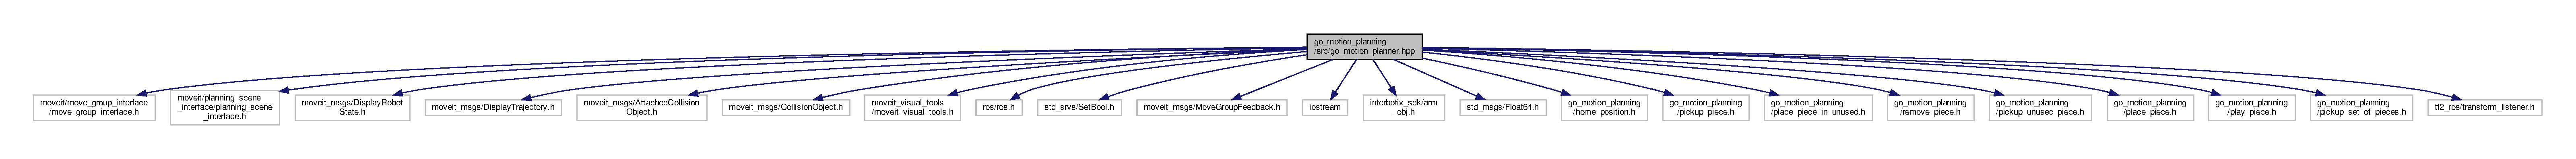
\includegraphics[width=350pt]{go__motion__planner_8hpp__incl}
\end{center}
\end{figure}
This graph shows which files directly or indirectly include this file\+:\nopagebreak
\begin{figure}[H]
\begin{center}
\leavevmode
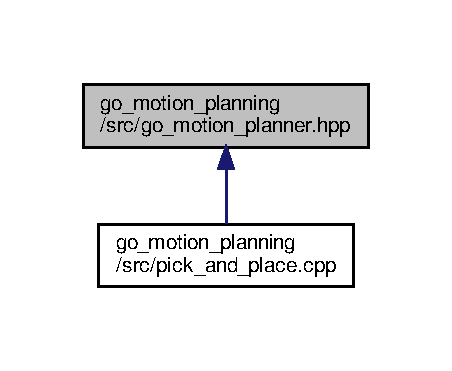
\includegraphics[width=217pt]{go__motion__planner_8hpp__dep__incl}
\end{center}
\end{figure}
\subsection*{Classes}
\begin{DoxyCompactItemize}
\item 
class \hyperlink{classgo__motion__planner}{go\+\_\+motion\+\_\+planner}
\begin{DoxyCompactList}\small\item\em Provides high level abstraction and motion planning services for the Go\+Bot. \end{DoxyCompactList}\end{DoxyCompactItemize}


\subsection{Detailed Description}
\hyperlink{classgo__motion__planner}{go\+\_\+motion\+\_\+planner} header declares a set of R\+OS services for picking and placing go\+\_\+pieces 

Parameters\+: /home\+\_\+position\+\_\+x -\/ Gripper frame\textquotesingle{}s pose x value in the home position /home\+\_\+position\+\_\+y -\/ Gripper frame\textquotesingle{}s pose y value in the home position /home\+\_\+position\+\_\+z -\/ Gripper frame\textquotesingle{}s pose z value in the home position /home\+\_\+position\+\_\+roll -\/ Gripper frame\textquotesingle{}s pose roll value (radians) in the home position /home\+\_\+position\+\_\+pitch -\/ Gripper frame\textquotesingle{}s pose pitch (radians) value in the home position /home\+\_\+position\+\_\+yaw -\/ Gripper frame\textquotesingle{}s pose yaw (radians) value in the home position

/row\+\_\+width -\/ The width of the go board\textquotesingle{}s square /row\+\_\+height -\/ The height of the go board\textquotesingle{}s square

/z\+\_\+board\+\_\+plane -\/ The z-\/axis value of the top of the board\textquotesingle{}s plane /piece\+\_\+height -\/ Height of the go piece /z\+\_\+stance\+\_\+offset -\/ The distance in the z-\/axis to be offset by in the stance pose /finger\+\_\+length -\/ The length of the gripper\textquotesingle{}s fingers

Publishes\+: /rx200/gripper\+\_\+controller/command -\/ Position controller of the robot\textquotesingle{}s gripper /rx200/gripper/command -\/ P\+WM control of the gripper

Subscribes\+: /rx200/gripper/command -\/ P\+WM control feedback from the gripper

Services\+: /home\+\_\+position -\/ Move robot into a home pose /pickup\+\_\+piece -\/ Pickup a piece at the given (row, column) pair /place\+\_\+piece\+\_\+in\+\_\+unused -\/ Place a piece in the used pile /remove\+\_\+piece -\/ Pickup and remove a piece at the given (row, column) from the board /pickup\+\_\+unused\+\_\+piece -\/ Pickup an unused piece from the empty pile /place\+\_\+piece -\/ Place a piece at the given (row, column) on the board /play\+\_\+piece -\/ Pickup an used piece and play it on the board at (row, column) /pickup\+\_\+set\+\_\+of\+\_\+pieces -\/ Pickup a set of pieces and remove them from the board 
\hypertarget{pick__and__place_8cpp}{}\section{go\+\_\+motion\+\_\+planning/src/pick\+\_\+and\+\_\+place.cpp File Reference}
\label{pick__and__place_8cpp}\index{go\+\_\+motion\+\_\+planning/src/pick\+\_\+and\+\_\+place.\+cpp@{go\+\_\+motion\+\_\+planning/src/pick\+\_\+and\+\_\+place.\+cpp}}


Service node to use Move\+It to pick and place go pieces.  


{\ttfamily \#include $<$moveit/move\+\_\+group\+\_\+interface/move\+\_\+group\+\_\+interface.\+h$>$}\newline
{\ttfamily \#include $<$moveit/planning\+\_\+scene\+\_\+interface/planning\+\_\+scene\+\_\+interface.\+h$>$}\newline
{\ttfamily \#include $<$moveit\+\_\+msgs/\+Display\+Robot\+State.\+h$>$}\newline
{\ttfamily \#include $<$moveit\+\_\+msgs/\+Display\+Trajectory.\+h$>$}\newline
{\ttfamily \#include $<$moveit\+\_\+msgs/\+Attached\+Collision\+Object.\+h$>$}\newline
{\ttfamily \#include $<$moveit\+\_\+msgs/\+Collision\+Object.\+h$>$}\newline
{\ttfamily \#include $<$moveit\+\_\+visual\+\_\+tools/moveit\+\_\+visual\+\_\+tools.\+h$>$}\newline
{\ttfamily \#include \char`\"{}go\+\_\+motion\+\_\+planner.\+hpp\char`\"{}}\newline
{\ttfamily \#include $<$tf2/\+Linear\+Math/\+Quaternion.\+h$>$}\newline
{\ttfamily \#include $<$tf2\+\_\+geometry\+\_\+msgs/tf2\+\_\+geometry\+\_\+msgs.\+h$>$}\newline
{\ttfamily \#include \char`\"{}actionlib\+\_\+msgs/\+Goal\+Status.\+h\char`\"{}}\newline
{\ttfamily \#include $<$tf/tf.\+h$>$}\newline
{\ttfamily \#include $<$std\+\_\+msgs/\+Float64.\+h$>$}\newline
{\ttfamily \#include \char`\"{}go\+\_\+motion\+\_\+planning/home\+\_\+position.\+h\char`\"{}}\newline
{\ttfamily \#include \char`\"{}go\+\_\+motion\+\_\+planning/pickup\+\_\+piece.\+h\char`\"{}}\newline
{\ttfamily \#include $<$math.\+h$>$}\newline
Include dependency graph for pick\+\_\+and\+\_\+place.\+cpp\+:\nopagebreak
\begin{figure}[H]
\begin{center}
\leavevmode
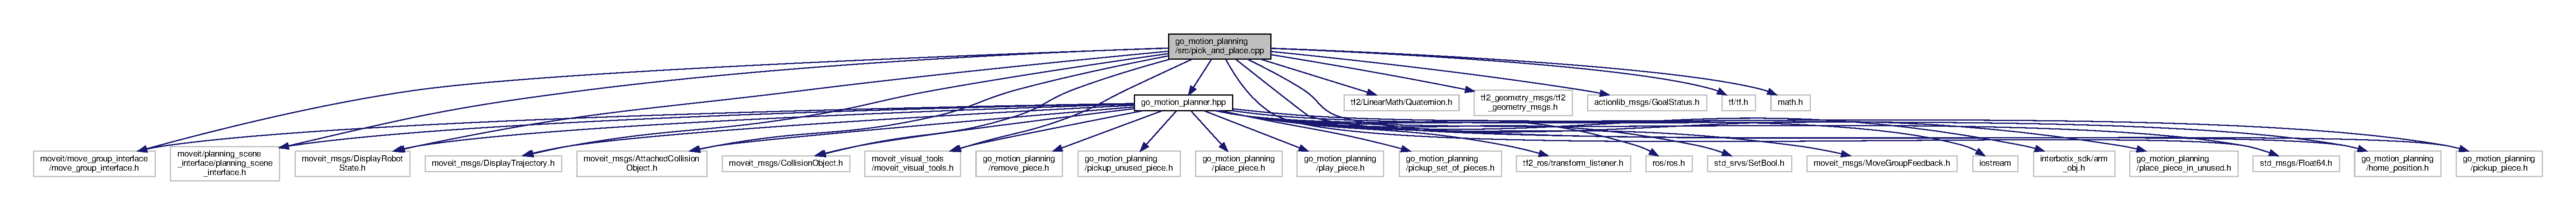
\includegraphics[width=350pt]{pick__and__place_8cpp__incl}
\end{center}
\end{figure}
\subsection*{Functions}
\begin{DoxyCompactItemize}
\item 
\mbox{\Hypertarget{pick__and__place_8cpp_a3c04138a5bfe5d72780bb7e82a18e627}\label{pick__and__place_8cpp_a3c04138a5bfe5d72780bb7e82a18e627}} 
int {\bfseries main} (int argc, char $\ast$$\ast$argv)
\end{DoxyCompactItemize}


\subsection{Detailed Description}
Service node to use Move\+It to pick and place go pieces. 

Parameters\+: /home\+\_\+position\+\_\+x -\/ Gripper frame\textquotesingle{}s pose x value in the home position /home\+\_\+position\+\_\+y -\/ Gripper frame\textquotesingle{}s pose y value in the home position /home\+\_\+position\+\_\+z -\/ Gripper frame\textquotesingle{}s pose z value in the home position /home\+\_\+position\+\_\+roll -\/ Gripper frame\textquotesingle{}s pose roll value (radians) in the home position /home\+\_\+position\+\_\+pitch -\/ Gripper frame\textquotesingle{}s pose pitch (radians) value in the home position /home\+\_\+position\+\_\+yaw -\/ Gripper frame\textquotesingle{}s pose yaw (radians) value in the home position

/row\+\_\+width -\/ The width of the go board\textquotesingle{}s square /row\+\_\+height -\/ The height of the go board\textquotesingle{}s square

/z\+\_\+board\+\_\+plane -\/ The z-\/axis value of the top of the board\textquotesingle{}s plane /piece\+\_\+height -\/ Height of the go piece /z\+\_\+stance\+\_\+offset -\/ The distance in the z-\/axis to be offset by in the stance pose /finger\+\_\+length -\/ The length of the gripper\textquotesingle{}s fingers

Publishers\+: /rx200/gripper\+\_\+controller/command -\/ Position controller of the robot\textquotesingle{}s gripper /rx200/gripper/command -\/ P\+WM control of the gripper

Subscribers\+: /rx200/gripper/command -\/ P\+WM control feedback from the gripper

Services\+: /home\+\_\+position -\/ Move robot into a home pose /pickup\+\_\+piece -\/ Pickup a piece at the given (row, column) pair /place\+\_\+piece\+\_\+in\+\_\+unused -\/ Place a piece in the used pile /remove\+\_\+piece -\/ Pickup and remove a piece at the given (row, column) from the board /pickup\+\_\+unused\+\_\+piece -\/ Pickup an unused piece from the empty pile /place\+\_\+piece -\/ Place a piece at the given (row, column) on the board /play\+\_\+piece -\/ Pickup an used piece and play it on the board at (row, column) /pickup\+\_\+set\+\_\+of\+\_\+pieces -\/ Pickup a set of pieces and remove them from the board 
%--- End generated contents ---

% Index
\backmatter
\newpage
\phantomsection
\clearemptydoublepage
\addcontentsline{toc}{chapter}{Index}
\printindex

\end{document}
